% !TeX spellcheck = de_DE
\documentclass{uebung_cs}
\usepackage{algo121}
\blattname{\emoji{star}-Aufgabe: Kreuzende Linien}

%%%%%%%%%%%%%%%%%%%%%%%%%%%%%%%%%%%%%%%%%%%%%%%%%%%%%%%%%%%%%%%%%%%%%%%%%%%%


\begin{document}
	Gegeben seien zwei Sequenzen von Punkten in der $xy$-Ebene, nämlich $p_1,\dots,p_n$ auf der Linie $y=0$ und $q_1,\dots,q_n$ auf der Linie $y=1$.
	Erzeuge nun $n$ Strecken, indem jeder Punkt $p_i$ mit $q_i$ verbunden wird.
	Beschreibe und analysiere einen \emph{divide-and-conquer} Algorithmus, der in Zeit $O(n \log n)$ ausrechnet, wie viele Paare von Strecken sich schneiden.

	Zum Beispiel gibt es unter den folgenden 7 Strecken genau 8 Paare von Strecken, die sich schneiden:
	\begin{center}
	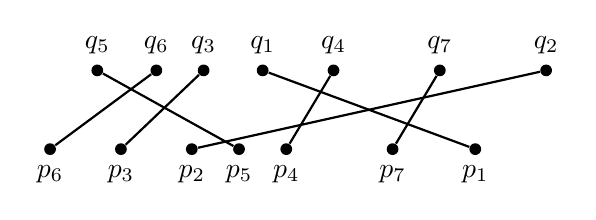
\begin{tikzpicture}[xscale=1.5]
		\node[fill,circle,inner sep=1.5pt,label=below:{$p_1$}] (p1) at (4,0) {};
		\node[fill,circle,inner sep=1.5pt,label=below:{$p_2$}] (p2) at (1.6,0) {};
		\node[fill,circle,inner sep=1.5pt,label=below:{$p_3$}] (p3) at (1,0) {};
		\node[fill,circle,inner sep=1.5pt,label=below:{$p_4$}] (p4) at (2.4,0) {};
		\node[fill,circle,inner sep=1.5pt,label=below:{$p_5$}] (p5) at (2,0) {};
		\node[fill,circle,inner sep=1.5pt,label=below:{$p_6$}] (p6) at (0.4,0) {};
		\node[fill,circle,inner sep=1.5pt,label=below:{$p_7$}] (p7) at (3.3,0) {};
		\node[fill,circle,inner sep=1.5pt,label=above:{$q_1$}] (q1) at (2.2,1) {};
		\node[fill,circle,inner sep=1.5pt,label=above:{$q_3$}] (q3) at (1.7,1) {};
		\node[fill,circle,inner sep=1.5pt,label=above:{$q_2$}] (q2) at (4.6,1) {};
		\node[fill,circle,inner sep=1.5pt,label=above:{$q_4$}] (q4) at (2.8,1) {};
		\node[fill,circle,inner sep=1.5pt,label=above:{$q_5$}] (q5) at (0.8,1) {};
		\node[fill,circle,inner sep=1.5pt,label=above:{$q_6$}] (q6) at (1.3,1) {};
		\node[fill,circle,inner sep=1.5pt,label=above:{$q_7$}] (q7) at (3.7,1) {};
		\foreach\i in {1,...,7} {
			\draw[thick] (p\i)--(q\i);
		}
	\end{tikzpicture}
	\end{center}
	
	Die Eingabe soll gegeben sein als zwei Felder $p[1..n]$ und $q[1..n]$ von ganzen Zahlen, sodass $p[i]$ die $x$-Koordinate von $p_i$ beschreibt und $q[j]$ die $x$-Koordinate von $q_j$. Sie dürfen annehmen, dass alle $x$-Koordinaten verschieden sind.

\paragraph{Spezielle Bewertungskriterien.}
Die Abgabe wird \emph{akzeptiert}, wenn die Aufgabe vollständig und korrekt gelöst wurde und dabei fast keine Abstriche in den allgemeinen Bewertungskriterien erkennbar sind.

\input{allgemeine-kriterien.inc}
\end{document}
